\documentclass[12pt]{exam}

\usepackage{amssymb}
\usepackage{mathtools}
\usepackage{algorithm}
\usepackage{float}  % Figure placement
\usepackage{minted}  % Code highlighting
\usepackage{tikz}  % Flow chart
\usepackage{lipsum}
\usepackage{xspace}
\usepackage{hyperref}
\usepackage{MnSymbol}
\usepackage{pgffor}



\hypersetup{
    colorlinks = true,
    linkcolor = blue,
    urlcolor  = blue,
    citecolor = blue,
    anchorcolor = blue
}

\newcommand{\hwheaderfooter}[3]{
\pagestyle{headandfoot}
\firstpageheadrule
\firstpageheader{#1}{#2}{#3}
\runningheader{#1}{#2}{#3}
\runningheadrule
\firstpagefooter{}{\thepage}{}
\runningfooter{}{\thepage}{}
}

\newcommand{\latex}{\LaTeX\xspace}

\newcommand{\stars}[1]{%
    \foreach \n in {1,...,#1}{%
        $\filledstar$%
    }%
}

\usetikzlibrary{shapes.geometric, arrows}
\tikzstyle{arrow} = [thick,->,>=stealth]

\hwheaderfooter{HW 3}{Ching}{CSCI 406}


\begin{document}
\begin{center}
    \fbox{\fbox{\parbox{\textwidth - 0.2 in}{\centering

                {Instructions: Please note that handwritten assignments \textbf{will not be graded}. Use the
                    provided \latex template to complete your homework. Please do not alter the order or spacing of
                    questions (keep each question on its own page). When you submit to Gradescope, you must mark
                    which page(s) correspond to each question. \textbf{You may not receive credit for unmarked
                        questions}. \\ When including graphical figures, we encourage the use of tools such as \href{https://dreampuf.github.io/GraphvizOnline/}{graphviz} or packages like \href{https://www.overleaf.com/learn/latex/TikZ_package}{tikz} for simple and complex figures. However, these may be handwritten only if they are neat and legible (as defined by the grader). }\\

            }}}
\end{center}

\textbf{List any collaborators (besides TAs or professors) here:}

\begin{questions}

    \question[9] [W3, \stars{2}] Topological Sort.
    For the following questions, select whether the statement is true or false,
    and write a \textit{brief} (approximately one sentence) explanation of your reasoning.

    \begin{parts}
        \part The DFS-based topological sort algorithm we discussed in class uses vertex
        start times computed during a DFS traversal of the given DAG.

        % Replace \square with \blacksquare for the option you would like to select.
        $\square$ True $\blacksquare$ False

        The DFS-based topological sort algorithm uses finish times, not start times, computed during a DFS traversal of the given Directed Acyclic Graph (DAG).

        \part Topological Sort is $\mathcal{O}(E + V \log V)$, due to needing to sort the vertices by finish time
        ($V$ is the number of vertices, $E$ the number of edges).

        % Replace \square with \blacksquare for the option you would like to select.
        $\square$ True $\blacksquare$ False

        The time complexity of the standard DFS-based topological sort is $\mathcal{O}(E + V)$, as it is a DFS traversal of the graph. The need for sorting the vertices is not a part of the standard topological sort algorithm.

        \part After a topological sort has been performed, a topological order starts with a vertex that has no incoming edges (that is, in-degree of zero).

        $\blacksquare$ True $\square$ False

        After a topological sort has been performed, the order starts with a vertex that has no incoming edges, meaning it has an in-degree of zero. This is a property of a valid topological order in a Directed Acyclic Graph (DAG).

    \end{parts}
    \clearpage

    \question[15] [W3, \stars{2}] Perform toposort using a DFS

    \begin{figure}[h]
        \center
        \includegraphics[width = 3in]{./flowchart.pdf}
    \end{figure}


    \begin{parts}

        \part Perform a DFS on the DAG in the figure above. Write the start and finish timestamps of each of the
        vertices.

        \begin{tabular}{l|c|c}
            \textbf{Vertex} & \textbf{Start Timestamp} & \textbf{Finish Timestamp} \\
            261             & 1                        & 14                        \\
            262             & 2                        & 13                        \\
            306             & 9                        & 10                        \\
            341             & 5                        & 8                         \\
            358             & 15                       & 16                        \\
            403             & 11                       & 12                        \\
            406             & 3                        & 4                         \\
            442             & 6                        & 7
        \end{tabular}

        \item List the vertices in topological order based on the
        times above.

        \begin{tabular}{c}
            358, 261, 262, 403, 306, 341, 442, 406
        \end{tabular}

        \item List an alternative topological ordering of the DAG above. (It does not have to be based on another DFS. Any valid ordering is acceptable.)

        \begin{tabular}{c}
            261, 358, 262, 403, 306, 341, 442, 406
        \end{tabular}

        I just swapped the first two vertices in the previous topological order.

    \end{parts}

    \clearpage

    \question[10] [W3, \stars{2}] Draw a graph with 7 vertices and any number of edges such that there are 720 possible topological orderings. Provide a \textit{brief} (approximately 2 sentence) explanation of your solution.

    \begin{figure}[H]
        \center
        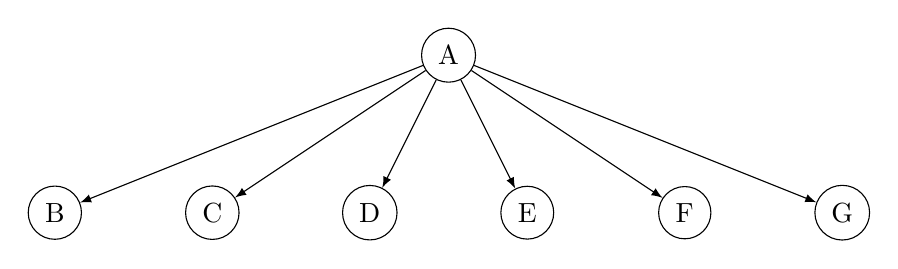
\begin{tikzpicture}[>=latex]
            % Create a node 1 with 6 branches
            \node[draw, circle] (1) at (7, 2) {A};
            \node[draw, circle] (2) at (2, 0) {B};
            \node[draw, circle] (3) at (4, 0) {C};
            \node[draw, circle] (4) at (6, 0) {D};
            \node[draw, circle] (5) at (8, 0) {E};
            \node[draw, circle] (6) at (10, 0) {F};
            \node[draw, circle] (7) at (12, 0) {G};

            % Draw arrows between the nodes
            \draw[->] (1) -- (2);
            \draw[->] (1) -- (3);
            \draw[->] (1) -- (4);
            \draw[->] (1) -- (5);
            \draw[->] (1) -- (6);
            \draw[->] (1) -- (7);
        \end{tikzpicture}
    \end{figure}

    \textbf{Explanation:} For every possible topo ordering, the first node is 'A'. The remaining nodes can be in any order, so there are $6! = 720$ possible orderings.

    \clearpage

    \question[9] [W4, \stars{2}] Articulation Vertices.
    For the following questions, select whether the statement is true or false,
    and write a \textit{brief} (approximately one sentence) explanation of your reasoning.

    \begin{parts}

        \part Consider unique vertices $u, v$, and $x$. If all paths between $u$ and $v$ include $x$, then $x$ is an articulation vertex.

        % Replace \square with \blacksquare for the option you would like to select.
        $\blacksquare$ True $\square$ False

        Removing $x$ would disconnect all paths from $u$ to $v$, so $x$ is an articulation vertex.

        \part An articulation vertex can have any degree $\geq 1$.

        % Replace \square with \blacksquare for the option you would like to select.
        $\square$ True $\blacksquare$ False

        An articulation vertex must have a degree $\geq 2$ in order to disconnect the graph when removed. A vertex with degree 1 cannot disconnect the graph when removed, it would just remove a leaf node.

        \part Consider a graph model of the internet where nodes are the various routers, servers, switches, devices, etc. that internet traffic can go through, and edges are connections between those network components. Assume all internet traffic from the Mines network goes through a single network switch in CTLM (there are no backup switches or alternative routes that internet traffic can take to exit the Mines network). The node representing that switch would be an articulation vertex in this model of the internet.

        % Replace \square with \blacksquare for the option you would like to select.
        $\blacksquare$ True $\square$ False

        Removing the switch would disconnect the Mines network from the rest of the internet, so the switch is an articulation vertex.

    \end{parts}
    \clearpage

    \question[10] [W4, \stars{2}] Strongly Connected Components.
    For the following questions, select whether the statement is true or false,
    and write a \textit{brief} (approximately one sentence) explanation of your reasoning.

    \begin{parts}
        \part If a new edge is added to a directed graph, the number of strongly connected components
        may \textbf{increase}.

        % Replace \square with \blacksquare for the option you would like to select.
        $\square$ True $\blacksquare$ False

        Can't increase the number of SCCs by adding an edge. Adding an edge can only decrease the number of SCCs or keep it the same.


        \part If a new edge is added to a directed graph, the number of strongly connected components
        may \textbf{decrease}.

        % Replace \square with \blacksquare for the option you would like to select.
        $\blacksquare$ True $\square$ False

        Adding an edge may decrease the number of strongly connected components. For example, adding an edge from c to b on the graph below would decrease the number of SCCs from 4 to 3.

        \textbf{SCC's:} $\{a,b,c,d,e\}, \{f,g\}, \{h\}$


        \part If a new edge is added to a directed graph, the number of strongly connected components
        may \textbf{stay the same}.

        % Replace \square with \blacksquare for the option you would like to select.
        $\blacksquare$ True $\square$ False

        Adding an edge may not change the number of strongly connected components. For example, adding an edge from b to c on the graph below would not change the number of SCCs.

        \textbf{SCC's:} $\{a,b,e\}, \{c,d\}, \{f,g\}, \{h\}$

    \end{parts}

    \vspace{1.5cm}
    \textbf{Example:}
    \begin{figure}[H]
        \centering
        \includegraphics[width=0.5\textwidth]{connected.png}
        \caption{Simple directed graph with 3 strongly connected components.}
    \end{figure}

    \textbf{SCC's:} $\{a,b,e\}, \{c,d\}, \{f,g\}, \{h\}$
    \clearpage


    \question[20] [W4, \stars{3}] Answer the following questions about Strongly Connected Components.
    \begin{parts}
        \part[10] What is the minimum number of edges in an SCC with $n$ vertices? Briefly describe how you
        would arrange the edges to create an SCC with $n$ vertices and a minimal number of edges (we are looking for approximately one sentence).

        \textbf{Min Edges:} $n$

        Create a cycle with $n$ vertices. Each vertex has an edge to the next vertex in the cycle. This creates an SCC with $n$ vertices and $n$ edges.

        \part[10] Prove that the SCC component graph (the graph with SCCs condensed to single vertices with edges between SCCs if there are edges between vertices in the original directed graph) is always a DAG. (Looking for approximately 1 paragraph.)

        The SCC component graph is always a DAG because the original graph is a DAG. In the SCC component graph, each SCC is a single vertex. If there is an edge between two SCCs, it means there is a path between some vertex in the first SCC and some vertex in the second SCC. Since the original graph is a DAG, there cannot be a cycle in the SCC component graph (otherwise it would merge the SCCs). Therefore, the SCC component graph is always a DAG.

    \end{parts}
    \clearpage

    \question[12] [W5, \stars{2}] MST.
    For the following questions, select whether the statement is true or false. \textbf{No explanation is necessary for these problems.}

    \begin{parts}
        \part Prim's and Kruskal's algorithms are both greedy algorithms.

        % Replace \square with \blacksquare for the option you would like to select.
        $\blacksquare$ True $\square$ False

        \part An MST of a graph is unique.

        % Replace \square with \blacksquare for the option you would like to select.
        $\square$ True $\blacksquare$ False

        \part In Kruskal's algorithm, it is correct to stop after adding
        $V - 1$ edges to the MST without considering the remaining edges.

        % Replace \square with \blacksquare for the option you would like to select.
        $\blacksquare$ True $\square$ False

        \part If an edge in the MST and another edge outside the MST have the same weight,
        replacing the edge inside the MST with the one outside yields another valid MST.

        % Replace \square with \blacksquare for the option you would like to select.
        $\square$ True $\blacksquare$ False

    \end{parts}
    \clearpage

    \question[15] [AlgoBOWL, \stars{2}] The following questions are about the AlgoBOWL project. For the following questions, select whether the statement is true or false. \textbf{No explanation is necessary for these problems.}

    \begin{parts}
        \part My team should expect to compute an optimal solution for every input with our algorithm.

        % Replace \square with \blacksquare for the option you would like to select.
        $\square$ True $\blacksquare$ False

        \part For an output from another team to be valid, it must match my team's output.

        % Replace \square with \blacksquare for the option you would like to select.
        $\square$ True $\blacksquare$ False

        \part The maximum number of edges in a prerequisite graph can be $n\cdot (n-1)$ for any $n$.

        % Replace \square with \blacksquare for the option you would like to select.
        $\blacksquare$ True $\square$ False

        \part Removing all vertices from the graph is a valid solution to the AlgoBOWL problem.

        % Replace \square with \blacksquare for the option you would like to select.
        $\blacksquare$ True $\square$ False


        \part If there are $k$ groups in your AlgoBOWL section (including your group), your group will
        need to:


        % Replace \square with \blacksquare for the option you would like to select.
        $\blacksquare$ Supply one input, compute $k$ outputs and perform $k$ verifications (not including open verification).\\
        $\square$ Supply one input, compute $k-1$ outputs and perform $k-1$ verifications (not including open verification).\\
        $\square$ Supply one input, compute $k$ outputs and perform $k^2$ verifications (not including open verification).\\
        $\square$ Supply one input, compute one output and perform one verification (not including open verification).

    \end{parts}

\end{questions}
\end{document}
